\documentclass[a4paper,11pt,titlepage]{article}

\usepackage[utf8]{inputenc}
\usepackage[T1]{fontenc}
\usepackage[english]{babel}
\usepackage{color}
\usepackage{xcolor}
\usepackage{graphicx}
\usepackage{amsmath}
\usepackage{amssymb}
\usepackage{mathtools}
\usepackage{stmaryrd}
\usepackage[hmargin={2.5cm,2.5cm},top=2.5cm,bottom=2.5cm]{geometry}
\usepackage{lmodern}
\usepackage[ruled,lined]{algorithm2e}
\usepackage{listings}
\usepackage{tikz, pgf}

\usepackage[colorlinks=true,breaklinks=true,linkcolor=blue,filecolor=magenta,urlcolor=cyan,pdftitle={Project},pdfsubject={Project}]{hyperref}

\usetikzlibrary{arrows,shapes,positioning}

\title{IA41 Project Template}
\author{blah}


\begin{document}
	
	\maketitle
	\newpage
	
	\tableofcontents
	\newpage
	
	\section{Introduction}
	
	\begin{align*}
		x = 2 &\implies x²=4 \text{ dtdtdtdt}
	\end{align*}
	
	\verb|azerxdrsdr5|
	
	
	\begin{center}
		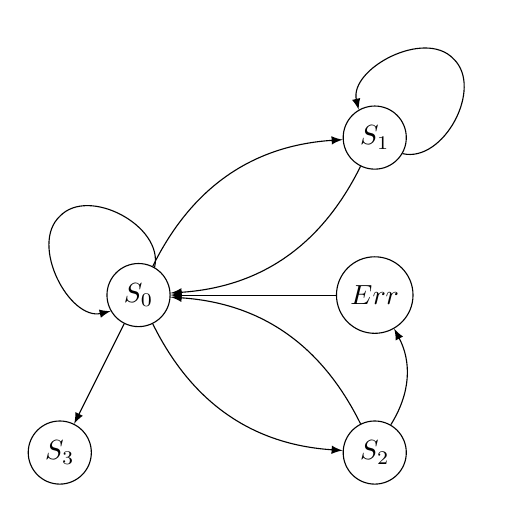
\begin{tikzpicture}
			\node[draw, circle] (S0) at (-1,0) {$S_0$} ;
			\node[draw, circle] (S1) at (2,2) {$S_1$} ;
			\node[draw, circle] (S2) at (2,-2) {$S_2$} ;
			\node[draw, circle] (S3) at (-2,-2) {$S_3$} ;
			\node[draw, circle] (Err) at (2,0) {$Err$} ;
			
			\draw (S0) to[bend right=75](-2,1);
			\draw[->,>=latex](-2,1) to[bend right=75](S0);
			
			\draw[->,>=latex] (S0) edge[bend left] (S1) ;
			\draw[->,>=latex] (S0) edge[bend right] (S2) ;
			\draw[->,>=latex] (S0) edge (S3) ;
			
			\draw[->,>=latex] (S1) edge[bend left] (S0) ;
			\draw (S1) to[bend right=75](3,3);
			\draw[->,>=latex](3,3) to[bend right=75](S1);
			
			\draw[->,>=latex] (S2) edge[bend right] (S0) ;
			\draw[->,>=latex] (S2) edge[bend right] (Err) ;
			
			\draw[->,>=latex] (Err) edge (S0) ;
		\end{tikzpicture}
	\end{center}
	
\end{document}
